\section{Begrüßung}

\begin{spacing}{1.4}
    \setlength{\parskip}{1.3ex}

    Hallo liebe Erstis,

    wir, der Fachschaftsrat, oder auch kurz FSR, 
    begrüßen euch ganz herzlich an der MLU.
    Mit unseren pinken T-Shirts sind wir den meisten 
    von euch ja schon bei den Erstiveranstaltungen begegnet.
    Neben der Erstiwoche sorgen wir während eurer gesamten Studienzeit
    für ein bisschen Spaß neben dem Alltagstrott, 
    stehen euch aber auch bei jeglichen Fragen zur Seite.
    Achtet auf unsere Nachrichten in der Studiengruppe und auf unsere Plakate für Spieleabende im Institut.
    Wir freuen uns, wenn ihr vorbeikommt!

    Als frisch gebackene Studierende seid ihr sicher gespannt, 
    was euch in den nächsten Monaten 
    an der Universität erwarten wird. 
    In den nächsten Wochen werdet ihr, 
    neben der ein oder anderen Ersti-Party,
    auch die ersten Vorlesungen und Übungen besuchen.

    Ganz schön viel Neues -- 
    aber zusammen mit euren KommilitonInnen 
    lassen sich die Übungsserien viel leichter stemmen.
    Und aus den anfänglichen Lerngruppen 
    können im Laufe der Zeit schnell FreundInnen fürs Leben werden.
    Ihr kommt mit den Übungen nicht klar? 
    Kommt mal in den Tutorien, 
    oder im Mathe-~oder Info-Treff vorbei, 
    wo euch andere Studis bei den Aufgaben unterstützen.

    Wir wünschen euch viel Spaß und Erfolg im Studium!

    Euer Fachschaftsrat \\
    \email{fachschaft@mathinf.uni-halle.de},
    Instagram: \email{@fsr.matheinfo.halle}
\end{spacing}
\vspace*{-1ex}
\begin{center}
    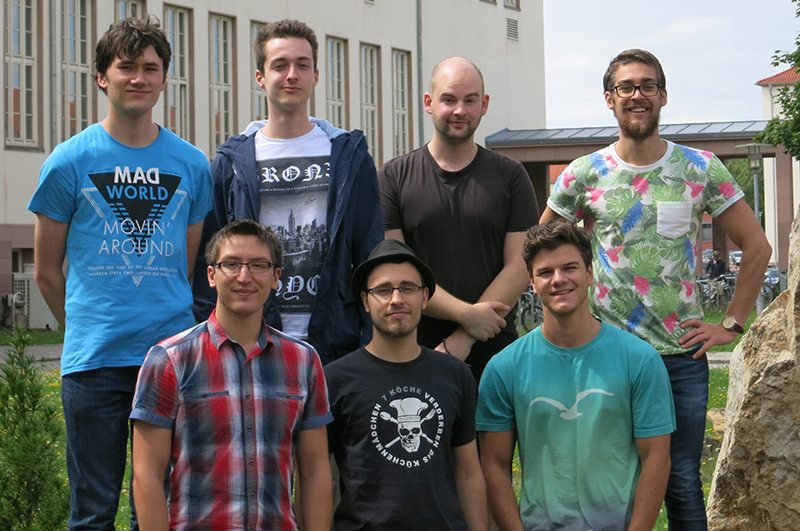
\includegraphics[width=1\linewidth]{fsr}
\end{center}%
FSR (v. l. n. r.): 
Erik Lange, Albert Arzumanian, Jonas Findeisen, Jan Heinrich Reimer, Willi Preuk, Anouk Ronja Océane Duyster, Fabian Kiesner, Aaron Gröbel, Patrick Tischendorf, Annemarie Bianka Weise, Sonne: Jan Moritz Mertens, Sonnenblume: Thi Kim Hanh Luu, Schildkröte: Lenz Hank-Weise 

